\section{Protocollo IP}
    
    I router determinano come instradare un pacchetto tramite lo strato di rete, il quale realizza \textit{consegne indirette}. I \textbf{router} sono componenti di rete molto semplici e veloci, e hanno l'unico scopo di far passare i pacchetti da una rete all'altra. 
    
    Un ritardo anche minimale su un router comporta ritardi in cascata su un intero percorso. Le \textbf{tavole di routing} indicano la strada in funzione dell'indirizzo di destinazione. 
    
    
    \begin{itemize}
        \item
            \textbf{Sul nodo mittente}, lo strato di rete ha la responsabilità di creare un pacchetto con i dati in arrivo da un protocollo degli strati superiori. L'intestazione del pacchetto contiene, fra le altre cose, l'indirizzo logico del mittente e quello del destinatario. 
            
            Lo strato di rete deve controllare la tavola di routing e trovare l'informazione necessaria, come ad esempio l'interfaccia di uscita sulla quale il pacchetto dev'essere spedito. Se il pacchetto è molto grande, lo si dovrà frammentare.
            
        \item
            \textbf{Sul router}, lo strato di rete ha la responsabilità di estrarre i dati dal pacchetto in arrivo (al fine di consultare la tavola di routing) e inoltrare il pacchetto verso la destinazione sull'interfaccia giusta. L'intestazione del pacchetto viene modificata.
                
        \item
            \textbf{Sul nodo destinatario}, lo strato di rete ha la responsabilità di verificare l'indirizzo di destinazione del pacchetto in arrivo, cioè controllare che il pacchetto sia arrivato alla destinazione corretta. Se il pacchetto è frammentato, lo stato di rete attende la ricezione di ogni frammento, per poi riassemblare il pacchetto originale.
    \end{itemize}
    
    L'infrastruttura Internet utilizza la commutazione di pacchetto con approccio a datagram per operare la commutazione nello strato di rete. La consegna datagram può essere svolta tramite un servizio orientato o meno alla connessione.
    
    \vspace{3mm}
    
    I \textbf{servizi orientati alla connessione} prevedono di instaurare una connessione prima della trasmissione dei dati, e cioè prestabilire un percorso ed elaborare una relazione logica fra i pacchetti inviati su tale percorso. La connessione viene eliminata a consegna avvenuta.
    
    I \textbf{servizi non orientati alla connessione} prevedono che i pacchetti seguano percorsi diversi per arrivare a destinazione, attraversando la rete in maniera disordinata e indipendente. Il servizio di comunicazione nello strato di rete di Internet è senza connessione.
    
    \vspace{3mm}
    
    IPv4 è uno dei principali protocolli della suite TCP/IP ed è detto "best-effort", e cioè non garantisce la consegna dei pacchetti. Implementa il servizio di consegna dei pacchetti senza connessione. Se si vuole affidabilità, bisogna affidarsi al TCP.
    
    \subsection{Formato dei datagram}
    
    I pacchetti del protocollo IP vengono detti datagram, composti da intestazione (20-60 byte) e dati (20-$2^31 - 1$ byte).
    
    \begin{center}
        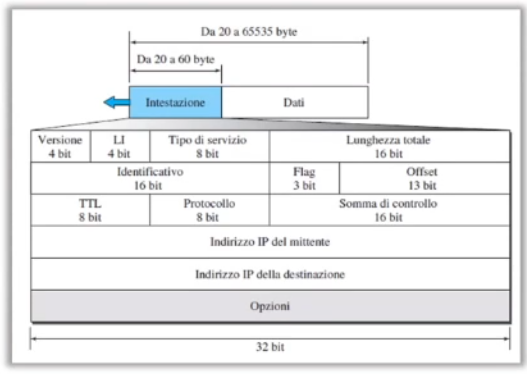
\includegraphics[scale=0.5]{images/IPv4.png}
    \end{center}
    
    \begin{itemize}
        \item 
            \textbf{Versione (4 bit).} Contiene il valore 4 (poiché stiamo esaminando l'IPv$4$; il valore sarebbe stato 6 nel caso dell'IPv$6$).
            
        \item 
            \textbf{Lunghezza intestazione (4 bit).} Indica la lunghezza totale dell'intestazione del datagram, misurata in parole di 4 byte (ogni bit rappresenta il valore di un byte, cioè 20-60 in binario).
            
        \item 
            \textbf{Tipo di servizio (8 bit).} Specifica come il pacchetto debba essere trattato. I primi 3 bit specificano la priorità del pacchetto (per questioni di congestione). I restanti bit indicano il servizio, i cui possibili valori sono \textit{R} (minimizza il ritardo), \textit{T} (massimizza il thoughput), \textit{A} (massimizza l'affidabilità) e \textit{C} (minimizza il costo). Sono valori mutualmente esclusivi (su 4 bit, solo uno varrà 1).
            
        \item 
            \textbf{Lunghezza totale (16 bit).} Analogo alla lunghezza dell'intestazione. Questa misura include la lunghezza dell'intestazione. Quest'informazione, intuitivamente inutile dato che ci basta valutare la dimensione del frame, risulta invece essenziale poiché all'interno del pacchetto potrebbero esserci dei byte di padding, cioè valori di riempimento per aumentare la dimensione del datagram. 
            
        \item 
            \textbf{Identificativo (16 bit).} Utilizzato per la frammentazione. Permette di individuare tutti i frammenti di un datagram.
            
        \item 
            \textbf{Flag (3 bit).} Utilizzato per la frammentazione. Il primo bit è riservato. Il secondo bit è di "\textit{non frammentazione}": se vale 1, il datagram non dev'essere frammentato. Il terzo bit è di "\textit{
altri frammenti}": se vale 1, significa che esitono altri frammenti del datagram (e cioè non ho finito di riassemblare questo stesso datagram).
            
        \item 
            \textbf{Offset (13 bit).} Utilizzato per la frammentazione. Indica lo spiazzamento, misurato in gruppi di 8 byte, e indica la posizione dei dati del frammento rispetto al datagram originale.
            
        \item 
            \textbf{Time-To-Live (8 bit).} L'IP prevede che un datagram abbia un tempo di vita limitato all'interno della rete. Se non raggiunge la destinazione entro il tempo limite, il datagram va distrutto. Rappresenta, in effetti, il numero massimo di router che il datagram può attraversare prima di giungere a destinazione. Il router si limiterà a decrementare un contatore.
            
        \item 
            \textbf{Protocollo (8 bit).} Definisce i protocolli degli strati superiori che stanno attualmente usando i servizi offerti dall'IP. E' importante per capire a quale protocollo devono essere consegnati i dati alla destinazione (ad esempio, TCP vale 6; ICMP vale 1; IGMP vale 2; UDP vale 17; OSPF vale 89).
            
        \item 
            \textbf{Somma di controllo (16 bit).} Rileva errori nell'intestazione. Inizialmente, viene posto a 0. L'intera intestazione viene suddivisa in blocchi di 16 bit, e la somma di questi blocchi (in complemento a 1) è proprio la somma di controllo.
            
        \item 
            \textbf{Indirizzo dell'host mittente (32 bit).} Rimane inalterato durante il viaggio.
            
        \item 
            \textbf{Indirizzo dell'host destinatario (32 bit).} Rimane inalterato durante il viaggio. Nello strato di collegamento, invece, l'indirizzo fisico mittente-destinatario cambia ad ogni nodo attraversato (cioè \textit{di hop in hop}).
            
        \item
            \textbf{Opzioni (al più 40 byte).} E' una parte non strettamente necessaria. Significa che se un datagram viene spedito con un campo Opzioni vuoto, non sarà scartato. Come suggerisce il nome, sono in genere usate per debugging e testing della rete: ad esempio, si possono specificare delle opzioni per instradare il datagram secondo un percorso guidato (e cioè tramite specifici router); registrare il percorso o, ancora, suggerirne uno in maniera indicativa. E' anche possibile memorizzare l'orario in cui un determinato datagram viene processato.
    \end{itemize}
    
    \subsection{Frammentazione dei datagram}
    
        Un datagram, per arrivare a destinazione, attraversa varie reti. Ogni router estrae il datagram IP dal frame nel quale esso arriva, lo analizza e (nella maggior parte dei casi) lo incapsula in un altro frame per rispedirlo. Il formato e la grandezza del frame nel quale il datagram viene incapsulato dipendono dalla rete nella quale il frame dovrà viaggiare.
        
        \begin{center}
            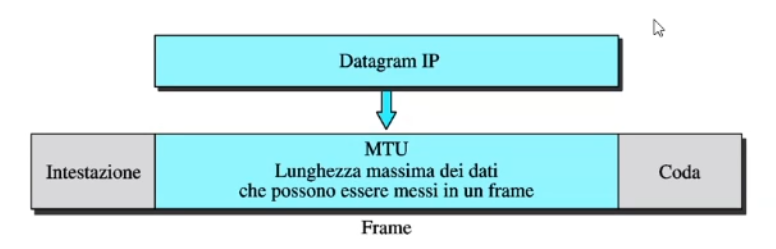
\includegraphics[scale=0.5]{images/MTU.png}
        \end{center}
        
        La dimensione massima dei dati in un frame è denotata con MTU (Maximum Transfer Unit), e varia da rete a rete. Nel caso di Internet, l'MTU è di 1500 byte. Ciò significa che se un datagram ha una dimensione maggiore di 1500 byte, dovrà essere frammentato e riassemblato all'avvio.
        
        \vspace{3mm}
        
        La \textbf{frammentazione} può avvenire già nel nodo sorgente. Il singolo frammento è esso stesso un datagram; inoltre, il riassemblaggio può avvere solo nella destinazione. Ricordiamo che alcuni dati del datagram IP sono coinvolti nella frammentazione. Tali dati concorronno al riassemblaggio.
        
        Per poter riassemblare i frammenti, la destinazione identifica il primo frammento cercando l'offset pari a 0. La lunghezza del primo frammento, divisa per 8, fornisce il valore dell'offset che deve avere il secondo frammento. Il processo continua in questo modo fin quanto si arriva ad un frammento in cui il valore del bit "\textit{di altri frammenti}" è 0.